\section{Software architecture}\label{sec:architecture}
% Sources: OUTLINE.md §4; dossier 02 §1, §7, §8; dossier 03 §1, §3–§5, §7–§10, §12.
% Code anchors are in the main repository (branch phase-2-cr-acceptance); re-anchor at the release commit.

\subsection{Design rules}\label{sec:arch-rules}

Nine design rules fix the shape of the package. % [R] SPEC.md §3 (R1–R9)
Five shape the interface: composition over inheritance (R1: a model is \code{BVAR(mean, vol, ...)},
with no model-specific classes), volatility first (R2), one predictive contract for both engines
(R3), the variable ordering surfaced rather than hidden (R8), and no look-ahead (R9: everything
data-dependent is recomputed inside each estimation window).
Three govern the internals: float64 throughout, no explicit inverses, precision-based samplers and
log-space densities (R4); no sampler merged without passing Geweke and simulation-based calibration
tests (R6; \cref{sec:validation}); and one MCMC backend, hand-written Gibbs kernels in JAX
\citep{bradbury2018jax,frostig2018compiling} with no probabilistic programming language in the core
(R7).
R5 concerns licensing (\cref{sec:related}).
\cref{fig:architecture} shows the resulting layers.

\begin{figure}[tbp]
  \centering
  % Static figure; script docs/paper/figures/make_fig_architecture.py (OUTLINE §14, Fig1; naming per figures/make_common.py).
  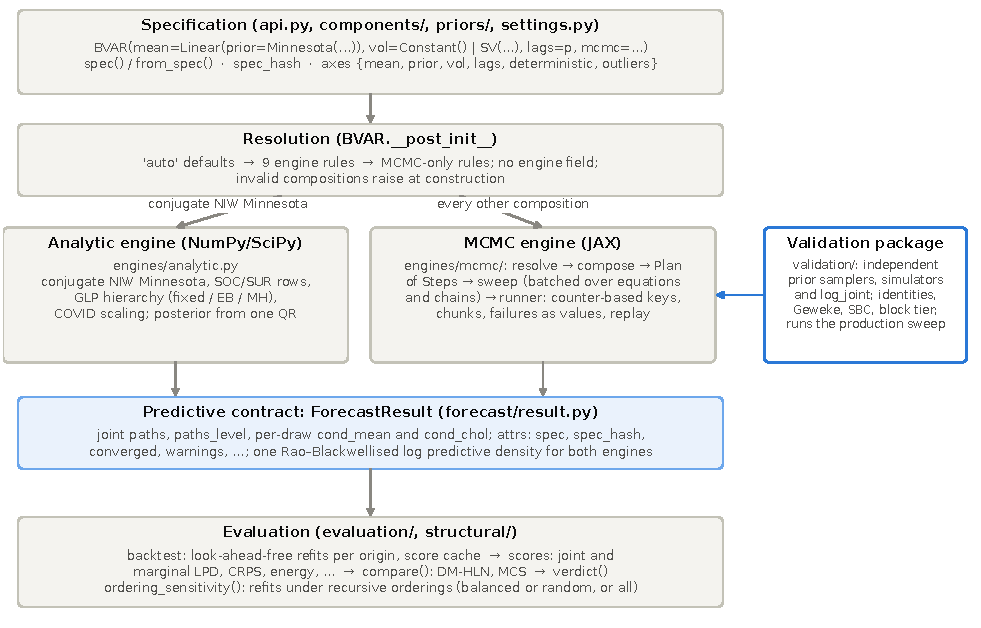
\includegraphics[width=\textwidth]{figures/fig_architecture.pdf}
  \caption{Architecture of \pkg{rai-bvar}. Specifications and engine resolution select the analytic
    (NumPy/SciPy) or the MCMC (JAX) engine. Both return the same \code{ForecastResult} contract, which
    feeds the backtest, the scores, \code{compare()} and \code{verdict()}. The validation package
    wraps the production sweep.}
  \label{fig:architecture}
\end{figure}

\subsection{Composition and engine resolution}\label{sec:arch-resolution}

A model is a frozen dataclass \code{BVAR(mean, vol, lags, deterministic, outliers, mcmc)} with no
engine field.
Its constructor resolves the \code{"auto"} defaults (a Minnesota form left at \code{"auto"} becomes
\code{"conjugate"} with a \code{Constant} prior left at \code{"auto"} or set to \code{"iw"}, and
\code{"structural"} otherwise; \code{Constant("auto")} then becomes \code{"iw"} or \code{"ig"}), applies the nine rules of \cref{tab:resolution}, and,
for MCMC compositions, rejects what the engine does not support: Lenza--Primiceri scaling and the
Metropolis--Hastings hyperparameter hierarchy (both planned for a later phase), and empirical Bayes
over $\psi$ with cross-lag tightness $\kappa_c \neq 1$ in structural form. % [R] src/rai_bvar/api.py (_check_mcmc_rules error messages: "arrives in Phase 3")
Every error is raised at construction. A parametrised test encodes the seven non-error rows of the
table case by case, and further tests check each construction error with its
message. % [V] src/rai_bvar/api.py (BVAR.__post_init__, _resolve_auto, _check_mcmc_rules); tests/unit/test_api_resolution.py::test_resolution_table (rows 1, 3–8), ::test_conjugate_form_with_any_other_volatility_raises (row 2), ::test_reduced_form_with_the_conjugate_iw_prior_raises (row 9), ::test_lenza_primiceri_scaling_is_rejected_on_mcmc, ::test_metropolis_hastings_hierarchy_is_rejected_on_mcmc, ::test_structural_eb_over_psi_with_cross_shrinkage_is_rejected
Because the resolved components are stored, \code{BVAR()} keeps the meaning and hash it had before
the MCMC engine existed. % [V] tests/unit/test_phase1_hash_golden.py::test_default_spec_is_byte_identical_to_phase1, ::test_auto_defaults_resolve_to_the_phase1_composition

\begin{table}[tbp]
  \centering
  \small
  % Content read from src/rai_bvar/api.py (_resolve_auto, engine); cross-checked by
  % docs/paper/figures/tab_resolution.py against tests/unit/test_api_resolution.py::test_resolution_table (OUTLINE §14, Tab2).
  \begin{tabular}{@{}rllp{0.43\textwidth}@{}}
    \toprule
    \# & Prior form & Volatility & Engine and mode \\
    \midrule
    1 & conjugate  & \code{Constant("iw")}            & analytic (conjugate NIW) \\
    2 & conjugate  & any other                        & \code{ValueError} \\
    3 & structural & \code{Constant("ig")}            & MCMC, Mode~I \\
    4 & structural & \code{Constant("iw")}            & MCMC, Mode~II (NIW twin); prior label \code{scaling=conjugate} \\
    5 & structural & \code{Constant("iw\_equivalent")} & MCMC, Mode~I $\delta$ prior with the $(a, \lambda)$ prior of \citet{chan2022asymmetric} \\
    6 & structural & \code{SV(...)}                   & MCMC, Mode~I \\
    7 & reduced    & \code{Constant("ig")}, \code{SV(...)} & MCMC, corrected triangular (CCCM) step \\
    8 & reduced    & \code{Constant("iw\_equivalent")} & MCMC, CCCM step with Chan's $(a, \lambda)$ prior; order-invariant \\
    9 & reduced    & \code{Constant("iw")}            & \code{ValueError} \\
    \bottomrule
  \end{tabular}
  \caption{Engine resolution: the rules that map a resolved (prior form, volatility prior) to an engine
    and mode. The first match applies, and errors are raised at construction. \code{BVAR()},
    \code{BVAR(vol=Constant("ig"))} and \code{BVAR(vol=SV())} reach rules 1, 3 and 6.}
  \label{tab:resolution}
\end{table}

\code{spec()} returns plain JSON, \code{from\_spec(spec())} round-trips (a property-based test), and a
golden test checks that every Phase~1 (conjugate) model keeps the specification hash, name and axes
recorded with the Phase~1 code. % [V] tests/unit/test_spec_roundtrip_mcmc.py::test_from_spec_inverts_spec_for_random_mcmc_compositions (hypothesis); tests/unit/test_phase1_hash_golden.py::test_phase1_models_keep_their_spec_hash_name_and_axes (values recorded at cbfcc5b)
The property \code{axes} splits a model into mean, prior, volatility, lags, deterministic terms and
outliers, and each axis label encodes every non-default setting, so ``differs along exactly one
axis'' is a property that \code{compare()} checks (\cref{sec:eval-verdict}).
Mode~II changes the mean prior, so its label carries \code{scaling=conjugate}, and it is never paired
with a Mode~I model along the volatility axis. % [V] tests/unit/test_api_resolution.py::test_mode_two_prior_axis_carries_the_conjugate_scaling
\code{import rai\_bvar} imports no JAX, which a subprocess test checks; the MCMC engine is loaded at
the first MCMC fit. % [V] tests/mcmc/unit/test_import_no_jax.py; tests/unit/test_api_resolution.py::test_mcmc_compositions_are_built_and_described_without_jax

\subsection{The analytic engine}\label{sec:arch-analytic}

The conjugate engine uses NumPy \citep{harris2020array} and SciPy \citep{virtanen2020scipy}.
One QR decomposition of the stacked Minnesota dummy rows, SOC/SUR rows and data gives the posterior;
$(R^\top R)^{-1}$ is never formed, and draws use the Bartlett decomposition.
Empirical Bayes maximises the log marginal likelihood plus the log hyperprior by L-BFGS-B, and the
hierarchical option is the random-walk Metropolis--Hastings scheme of \citet{giannone2015prior}. % [V] src/rai_bvar/engines/analytic.py (dossier 02 §5.1, §5.3)
The engine also computes recursive impulse responses and the forecast-error variance decomposition.

\subsection{The MCMC engine in six ideas}\label{sec:arch-mcmc}

\begin{enumerate}
  \item \emph{The static/traced split is the compilation cache key.} Choices that fix a shape or a
    branch live in a frozen, hashable \code{StaticConfig}; data, priors, hyperparameters, seeds and
    the sample length are traced. Time is padded, by default to $T_{\mathrm{pad}} = 32\lceil T/32\rceil$, with
    zero-weight rows, masked before any logarithm, so backtest windows in one bucket share compiled
    programs; a test of two such windows sees no recompilation. % [V] src/rai_bvar/engines/mcmc/config.py; tests/mcmc/runner/test_recompile.py::test_zero_recompiles_across_windows_of_one_bucket (runner toys)
  \item \emph{Equations and chains are \code{vmap} axes.} Given the volatilities the structural
    equations are conditionally independent, so kernels are written for one equation and batched,
    and the batched phase is an exact Gibbs block. Chains run under \code{vmap} (the default),
    \code{lax.map} or \code{shard\_map}.
  \item \emph{The Gibbs order is data.} A \code{Plan} of \code{Step}s with declared read and write sets
    is built in one function and printed by \code{fit.plan.describe()}. Invariants are checked for every
    composition, including a tree diff showing that each step writes only what it declares. The mixture
    indicators are local to the volatility step and never part of the state, so the rule of
    \citet{delnegro2015time} that nothing is drawn between the indicators and the log volatilities
    holds by construction. % [V] tests/mcmc/runner/test_plan.py::test_plan_invariants_every_composition_with_tree_diff, ::test_plan_invariants_production_kernels, ::test_tree_diff_catches_undeclared_write
  \item \emph{Kernels are pure and take injected noise:} \code{sample\_core(draw\_noise(key, ...), ...)}.
    Every exact draw exposes its conditional and every Metropolis--Hastings step its log acceptance
    ratio; the density-ratio identity tests of \cref{sec:validation} use both, and the failure
    replay evaluates the exposed conditionals. % [R] DESIGN §3.1 rules 2–3; [V] e.g. tests/mcmc/blocks/test_sv_core.py::test_exact_h_log_accept_identity
  \item \emph{Randomness is counter-based} \citep{salmon2011parallel}. Keys are \code{fold\_in} chains
    over stream, data salt, chain, absolute sweep, block, equation and sub-draw, with unsigned 32-bit
    counters and no key in any loop carry, so a draw depends on its position in the chain and not on
    how sweeps are grouped into compiled calls. % [V] src/rai_bvar/engines/mcmc/keys.py; tests/mcmc/runner/test_sweep.py::test_counter_must_be_uint32
  \item \emph{Failures are values.} Nothing raises inside compiled code and no jitter is added. Each
    chain keeps its first failure as $(\text{code}, it)$, with $\text{code} = 1 + 1000\cdot\text{block} +
    \text{equation}$; the host replays the failing chunk deterministically, evaluates the failing
    block's exposed conditional, and raises \code{MCMCNumericalError} with the block, equation,
    iteration and diagnostics. No chain is dropped. % [V] tests/mcmc/runner/test_failures.py::test_failure_in_burn_in_is_replayed, ::test_failure_in_sampling_is_replayed, ::test_replay_of_an_equation_failure_after_the_production_cccm_step
    \cref{sec:robustness} describes failures that surfaced this way.
\end{enumerate}

\subsection{Settings and runtime}\label{sec:arch-settings}

\code{MCMCSettings} is part of the specification: by default 4 chains of 2000 kept draws after a burn-in
of 1000, with convergence thresholds $\hat R < 1.01$ and bulk ESS $> 400$ on every primary monitored
quantity. % [V] src/rai_bvar/settings.py (MCMCSettings fields and docstring)
\code{Runtime} is not: it holds the device count (default 1), the kept draws per compiled call, a memory
budget that only decides whether to raise before sampling, a memory-mapped store, and whether the host
keeps replay copies. % [V] src/rai_bvar/settings.py (Runtime); tests/mcmc/runner/test_storage.py::test_run_raises_over_budget_before_sampling
The backtest never passes a \code{Runtime}, so cached scores do not depend on the machine's device
count. % [R] DESIGN §5.2; [V] src/rai_bvar/evaluation/backtest.py passes no Runtime
An \code{MCMCFit} holds the draws as an xarray \code{DataTree} \citep{hoyer2017xarray}, diagnostics,
a \code{summary()} (prior mode, hyperparameters, implied reduced-form prior moments, ordering), the
\code{converged} flag, \code{forecast()}, \code{irf()} and the final state for warm starts.

\subsection{Reproducibility, stated with its limits}\label{sec:arch-repro}

Bit-for-bit invariance is tested with the runner's test doubles (``toys'') for chunk and burn-in piece
size, aligned thinning, fused versus unfused plan execution, \code{vmap} over chains versus a loop, and
memory-mapped versus in-memory storage, and with the production kernels for chain-count prefixes under
\code{chains="map"}. % [V] tests/mcmc/runner/test_chunking.py::test_chunk_and_burn_piece_size_invariance, ::test_thinning_with_aligned_sweeps, ::test_mapped_chains_production_prefix; test_sweep.py::test_fused_equals_unfused_bitwise, ::test_vmap_over_chains_equals_sequential_loop; test_storage.py::test_memmap_store_equals_memory_store
With the production kernels, chain-count prefixes under \code{vmap} (SV and CCCM kernels) and
\code{vmap} versus \code{shard\_map} over four devices (structural SV) are equal only to rounding,
because XLA vectorises reductions differently for different batch sizes; the tests compare them to a
relative tolerance of $10^{-9}$ over a few burn-in sweeps. In-loop and post-hoc forecasts agree to
$10^{-12}$. % [V] test_chunking.py::test_production_chain_prefix_with_vmapped_chains_to_rounding (structural_sv), ::test_production_chain_prefix_with_vmapped_reduced_form_to_rounding (reduced_sv), 4-sweep burn; test_devices_bitwise.py::test_shard_map_matches_vmap_in_subprocess (structural_sv, 2-sweep burn); tests/mcmc/forecast/test_forecast_core.py::test_in_loop_forecast_equals_post_hoc_sv; [R] the XLA explanation: DESIGN §5.6 Stage 2 amendment
The toy chain-prefix test is bitwise on macOS and holds only to rounding on x86-64 Linux. % [V] test_chunking.py::test_chain_prefix_invariance (docstring)
Chunk invariance with the production kernels follows from the key layout but is not
tested,\todo{Dossier 03 Q17: add a production-kernel chunk test, or keep ``not tested''.} % [TC]
and nothing is guaranteed across platforms, JAX versions or PRNG implementations
(\cref{tab:TabG1} in \cref{app:repro}).
Every fit records the package and JAX versions, PRNG implementation, platform, device count, seed,
salt, resolved numerical paths, ordering and specification hash. % [V] src/rai_bvar/engines/mcmc/results.py (_metadata)
One hazard is avoided by layout: under partitionable threefry, words drawn directly from a parent key
equal the key data of its \code{fold\_in} children, which JAX's key-reuse checker cannot see. The key
layout therefore gives each consumer its own sub-key instead of drawing from a key whose children are
derived; a test checks this for the volatility core's forecast draws, where a draw from the block key
would reuse the words of the transitory sub-keys. % [R] DESIGN §3.1 rule 5, §5.6; [V] tests/mcmc/blocks/test_robust.py::test_ahead_and_transition_give_the_core_its_own_sub_key

\subsection{Extension protocol}\label{sec:arch-extension}

New components implement \code{MeanBlock}, \code{VolBlock}, \code{CoefPrior} or \code{GlobalStep} and
register an independent reference implementation, from which the validation package builds their
per-block and per-composition Geweke configurations. % [V] src/rai_bvar/engines/mcmc/protocols.py; src/rai_bvar/validation/reference.py (module docstring "Registry"; register_reference)
That later components will plug in without editing the sweep, runner or forecast core is a design
intention, not yet tested. % [R] DESIGN §3.9 (dossier 01, unsupported claim 3)
